\begin{document}

% ============================================
% SLIDE 1: Title
% ============================================
\begin{frame}
    \titlepage
\end{frame}

% ============================================
% SLIDE 2: Introduction & Motivation
% ============================================
\begin{frame}{Introduction \& Motivation}
    \begin{columns}
        \column{0.6\textwidth}
        \textbf{Star Sensors} are critical for spacecraft attitude determination:
        \begin{itemize}
            \item Capture images of star fields
            \item Identify stars and \textbf{compute their centroids}
            \item Match with star catalog for orientation (plate solving)
        \end{itemize}
        
        \vspace{0.5cm}
        \textbf{Key Requirements:}
        \begin{itemize}
            \item \textcolor{starblue}{\textbf{High accuracy}} — sub-pixel precision needed
            \item \textcolor{starblue}{\textbf{Fast computation}} — real-time processing
            \item \textcolor{starblue}{\textbf{Noise robustness}} — space environment challenges
        \end{itemize}
        
        \column{0.4\textwidth}
        \begin{tikzpicture}[scale=0.8]
            % Star field representation
            \fill[black] (0,0) rectangle (4,4);
            \foreach \x/\y/\s in {0.5/3.2/0.15, 1.2/2.5/0.2, 2.8/3.5/0.12, 
                                   3.2/1.8/0.18, 0.8/0.8/0.1, 2.2/1.2/0.25,
                                   3.5/2.8/0.08, 1.8/0.5/0.14} {
                \fill[stargold] (\x,\y) circle (\s);
            }
            \draw[white, thick] (2.2,1.2) circle (0.5);
            \draw[white, ->] (2.7,1.2) -- (3.5,1.2) node[right] {\tiny centroid};
        \end{tikzpicture}
    \end{columns}
\end{frame}


% ============================================
% SLIDE 3: Center of Gravity Method
% ============================================
\begin{frame}{Method 1: Center of Gravity (CoG)}
    \begin{columns}
        \column{0.55\textwidth}
        \textbf{Idea:} Weighted average of pixel positions by intensity
        
        \vspace{0.3cm}
        \begin{block}{CoG Formula}
            \[
            x_c = \frac{\sum_{i} I_{i} \cdot x_{i}}{\sum_{i} I_{i} }, \quad
            y_c = \frac{\sum_{j} I_{j} \cdot y_{j}}{\sum_{j} I_{j} }
            \]
        \end{block}
        
        \vspace{0.3cm}
        \begin{block}{Pros \& Cons}
            \begin{itemize}
                \item[\textcolor{green!60!black}{\checkmark}] \textbf{Very fast} — $O(n)$ computation
                \item[\textcolor{green!60!black}{\checkmark}] Simple to implement
                \item[\textcolor{red}{\texttimes}] \textbf{Sensitive} to background noise
                \item[\textcolor{red}{\texttimes}] Accuracy depends on window size
            \end{itemize}
        \end{block}
        
        \column{0.45\textwidth}
        \centering
        \begin{tikzpicture}[scale=0.6]
            % Grid
            \draw[gray, thin] (0,0) grid (5,5);
            % Star intensity (darker = brighter)
            \fill[stargold!20] (1,1) rectangle (2,2);
            \fill[stargold!30] (2,1) rectangle (3,2);
            \fill[stargold!20] (3,1) rectangle (4,2);
            \fill[stargold!40] (1,2) rectangle (2,3);
            \fill[stargold!90] (2,2) rectangle (3,3);
            \fill[stargold!40] (3,2) rectangle (4,3);
            \fill[stargold!20] (1,3) rectangle (2,4);
            \fill[stargold!30] (2,3) rectangle (3,4);
            \fill[stargold!20] (3,3) rectangle (4,4);
            % Centroid
            \fill[red] (2.5,2.5) circle (0.12);
            \node[below] at (2.5,0) {\small weighted average};
        \end{tikzpicture}
    \end{columns}
\end{frame}

% ============================================
% SLIDE 4: Gaussian Star Model
% ============================================
\begin{frame}{Gaussian Star Model}
    \textbf{Image Formation:} Any observed image is signal plus noise:
    \[
    I(x, y) = S(x, y) + N(x, y)
    \]
    where $S$ is the deterministic signal and $N$ is "random" noise.
    
    \vspace{0.3cm}
    \begin{block}{Star Image Model}
        The intensity distribution of a star can be modelled as a 2D Gaussian:
        \[
        S(x_i, y_i | v) = A \exp\left(-\frac{(x_i-x_c)^2}{2 \sigma_x^2} + \frac{(y_i-y_c)^2}{2\sigma_y^2}\right) 
        \]
        where v = $(A, x_c, y_c, \sigma_x, \sigma_y)$:
        \begin{itemize} 
            \item $(x_c, y_c)$ = star centroid (what we want to find)
            \item $A$ = Brightness of star (peak intensity)
            \item $\sigma_{x,y}$ = Standard deviation (spread)
        \end{itemize}
    \end{block}
    
    \vspace{0.3cm}
    \textbf{Challenge:} Stars span only a few pixels — need \textbf{sub-pixel accuracy}!
\end{frame}


% ============================================
% SLIDE 4': Gaussian Fitting Theory
% ============================================
\begin{frame}{Gaussian Fitting (GF): Formulation}
    \textbf{Objective:} Estimate star parameters $\mathbf{v}$ by fitting the Gaussian model $S$ to observed pixel intensities $I$.
    
    \vspace{0.2cm}
    \begin{block}{Objective Function (Least Squares)}
        \[
            Z = \operatorname*{argmin}_{\mathbf{v}} \sum_{(x_i, y_i) \in \mathcal{U}} \left( I(x_i, y_i) - S(x_i, y_i \mid \mathbf{v}) \right)^2
        \]
        where:
        \begin{itemize}
            \item $\mathcal{U}$ is the set of pixels in the star window
            \item $S(x_i, y_i \mid \mathbf{v})$ is the Gaussian model defined previously
            \item $\mathbf{v} = (A, x_c, y_c, \sigma_x, \sigma_y)$ are the optimization parameters
        \end{itemize}
    \end{block}

    \vspace{0.2cm}
    \textbf{Significance:}
    \begin{itemize}
        \item Provides the \textbf{Maximum Likelihood Estimation (MLE)} (under Gaussian noise).
        \item Theoretically the \textbf{most accurate} centroiding method.
    \end{itemize}
\end{frame}


% ============================================
% SLIDE 5: Gaussian Fitting Method
% ============================================
\begin{frame}{Gaussian Fitting: Implementation \& Challenges}
    \begin{columns}
        \column{0.55\textwidth}
        \textbf{Problem:} The model $S$ is \textbf{non-linear} with respect to positions $x_c, y_c$.
        
        \vspace{0.2cm}
        \textbf{Solution:} Iterative Numerical Optimization
        \begin{itemize}
            \item Algorithms: Levenberg-Marquardt, Trust-Region
            \item Requires complex iterative solvers
        \end{itemize}
        
        \vspace{0.2cm}
        \begin{block}{Pros \& Cons}
            \begin{itemize}
                \item[\textcolor{green!60!black}{\checkmark}] \textbf{Highest Accuracy}
                \item[\textcolor{green!60!black}{\checkmark}] Robust to pixel noise
                \item[\textcolor{red}{\texttimes}] \textbf{Computationally Expensive}
                \item[\textcolor{red}{\texttimes}] Requires good \textbf{initial guess} $\mathbf{v}_0$
                \item[\textcolor{red}{\texttimes}] \textbf{Instability:} May converge to local optima
            \end{itemize}
        \end{block}
        
        \column{0.45\textwidth}
        \centering
        \begin{tikzpicture}[scale=0.55, transform shape]
            % Axis
            \draw[->] (0,0) -- (5.2,0) node[right] {\Large $x$};
            \draw[->] (0,0) -- (0,4.2) node[above] {\Large $I$};
            
            % Model curve (Blue)
            \draw[starblue, very thick, domain=0:5, samples=60] 
                plot (\x, {3.5*exp(-(\x-2.5)^2/0.6)});
            \node[starblue] at (3.8, 3.5) {\Large $S(x \mid \mathbf{v})$};

            % Data points (Red)
            \foreach \x/\y in {0.5/0.1, 1/0.6, 1.5/2.1, 2/3.1, 2.5/3.4, 3/2.8, 3.5/1.9, 4/0.7, 4.5/0.2} {
                \fill[red] (\x,\y) circle (0.15);
                \draw[gray, thin, dashed] (\x,\y) -- (\x, {3.5*exp(-(\x-2.5)^2/0.6)});
            }
            
            % Centroid marker
            \draw[dashed, black] (2.5,0) -- (2.5,3.5);
            \node[below] at (2.5,-0.1) {\Large $x_c$};
        \end{tikzpicture}
        
        \vspace{0.3cm}
    \end{columns}
\end{frame}


% ============================================
% SLIDE 5: FGF Overview
% ============================================
\begin{frame}{Fast Gaussian Fitting (FGF): Formulation}
    \begin{columns}
        \column{0.6\textwidth}
        \textbf{Goal:} Overcome GF's computational cost while keeping high accuracy.
        
        \vspace{0.3cm}
        \textbf{Transformation:} Apply natural logarithm to the image model.
        \[
            g_i = \ln I(x_i, y_i) - \ln S(x_i, y_i)
        \]
        
        \textbf{New Objective Function ($G$):}
        \[
            G = \operatorname*{argmin}_{\mathbf{v}} \sum_{i \in \mathcal{U}} \left( \ln I_i - \ln S_i(\mathbf{v}) \right)^2 = \sum_{i \in \mathcal{U}} g_i^2
        \]
        \small \textit{(Minimizing log-difference instead of intensity difference)}
        
        \column{0.4\textwidth}
        \centering
        \begin{tikzpicture}[scale=0.7]
             \draw[->] (0,0) -- (3.5,0) node[right] {$x$};
             \draw[->] (0,0) -- (0,2.5) node[above] {$\ln I$};
             % Parabola
             \draw[thick, starblue] plot[domain=0.5:2.5] (\x, {2.2 - 2*(\x-1.5)^2});
             \node[align=center] at (1.5, -0.6) {Gaussian in log-domain\\becomes a \textbf{Parabola}};
        \end{tikzpicture}
    \end{columns}
    
    \vspace{0.2cm}
    \begin{alertblock}{Key Insight}
        This transforms the problem from \textbf{non-linear curve fitting} to \textbf{linear paraboloid fitting}, which has a direct analytic solution.
    \end{alertblock}
\end{frame}

% ============================================
% SLIDE 6: Linearization & Equivalence
% ============================================
\begin{frame}{Linearization \& Ideal Equivalence}
    \textbf{1. The Linear Model (Paraboloid):}
    By expanding $\ln S(x, y)$, we get a polynomial in $x, y$:
    \[
        \ln S(x, y) = a_0 + a_1 x + a_2 x^2 + a_3 y + a_4 y^2
    \]
    The star parameters $\mathbf{v}$ are recovered directly from coefficients $a_i$ using \textbf{Linear Least Squares}.

    \vspace{0.4cm}
    \textbf{2. Equivalence in Noise-Free Case ($N=0$):}
    If the image is perfect ($I = S$), minimizing the log-difference is identical to minimizing the intensity difference because $\ln(\cdot)$ is strictly monotonic.
    \[
        S(\mathbf{v}) = S(\mathbf{v}_{true}) \iff \ln S(\mathbf{v}) = \ln S(\mathbf{v}_{true})
    \]
    \textcolor{green!60!black}{\textbf{$\Rightarrow$ FGF yields the exact same result as GF when $N=0$.}}
\end{frame}

% ============================================
% SLIDE 7: Noise Sensitivity Analysis
% ============================================
\begin{frame}{Comparison: Noise Sensitivity Analysis}
    Substituting $I = S + N$ into the objective functions:
    
    \begin{columns}
        \column{0.55\textwidth}
        \textbf{1. GF (Standard):} Minimizes noise energy
        \[ Z \approx \operatorname*{argmin}_{\mathbf{v}} \sum [N_i]^2  \]
        
        \textbf{2. FGF (Log-domain):} Minimizes \textbf{weighted} noise
        \[ G \approx \operatorname*{argmin}_{\mathbf{v}} \sum [w_i N_i]^2 \]
        where weight $w_i = \frac{1}{N_i} \ln\left(1 + \frac{N_i}{S_i}\right) \approx \frac{1}{S_i}$
        
        \vspace{0.2cm}
        \textbf{Implication:}
        \begin{itemize}
            \item Lower Signal $S_i$ $\to$ \textbf{Higher Weight} $w_i$.
            \item \textbf{Edge pixels} are darker but have much larger weights.
        \end{itemize}
        
        \column{0.45\textwidth}
        \centering
        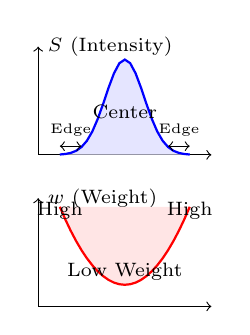
\begin{tikzpicture}[scale=0.55]
            % Intensity
            \begin{scope}[yshift=3.5cm]
                \draw[->] (0,0) -- (4,0);
                \draw[->] (0,0) -- (0,2.5) node[right] {\scriptsize $S$ (Intensity)};
                \draw[blue, thick, fill=blue!10] plot[domain=0.5:3.5] (\x, {2.2*exp(-(\x-2)^2/0.4)});
                \node at (2, 1) {\scriptsize Center};
                \draw[<->] (0.5, 0.2) -- (1, 0.2) node[midway, above] {\tiny Edge};
                \draw[<->] (3, 0.2) -- (3.5, 0.2) node[midway, above] {\tiny Edge};
            \end{scope}
            
            % Weight
            \begin{scope}
                \draw[->] (0,0) -- (4,0);
                \draw[->] (0,0) -- (0,2.5) node[right] {\scriptsize $w$ (Weight)};
                % Flattened parabola to fit inside axes (max y < 2.5)
                \draw[red, thick, fill=red!10] plot[domain=0.5:3.5] (\x, {0.5 + 0.8*(\x-2)^2}); 
                \node at (2, 0.8) {\scriptsize Low Weight};
                \node at (0.5, 2.2) {\scriptsize High};
                \node at (3.5, 2.2) {\scriptsize High};
            \end{scope}
        \end{tikzpicture}
    \end{columns}
    
    \vspace{0.2cm}
    \begin{block}{Conclusion}
         FGF is \textbf{biased towards noisy edge pixels}, making it more sensitive to noise than standard GF (which is not what we expect!).
    \end{block}
\end{frame}

% ============================================
% SLIDE 8: Addressing Weight Nonuniformity
% ============================================
\begin{frame}{Addressing Weight Nonuniformity}
    \textbf{Problem:} Previous analysis shows FGF is sensitive to edge noise due to nonuniform weights.
    
    \vspace{0.1cm}
    \textbf{Analysis:} Transform residual $g_i = \ln I_i - \ln S_i$ relative to noise $N_i$:
    \[
    g_i = \frac{N_i}{I_i} \cdot \varphi(r_i) \quad \text{with SNR } r_i = S_i / N_i
    \]

    \vspace{-0.1cm}
    \begin{columns}
        \column{0.5\textwidth}
        \textbf{Auxiliary Function:}
        \small
        \[
        \varphi(r_i) = (1 + r_i) \ln \left(1 + \frac{1}{r_i}\right)
        \]
        \normalsize
        \textbf{Behavior:}
        \small
        \begin{itemize}
            \item $|r_i| < 1$: Pixel is noise-submerged.
            \item $|r_i| > 1$: $\varphi(r)$ converges to 1.
        \end{itemize}
        \normalsize
        
        \column{0.4\textwidth}
        \centering
        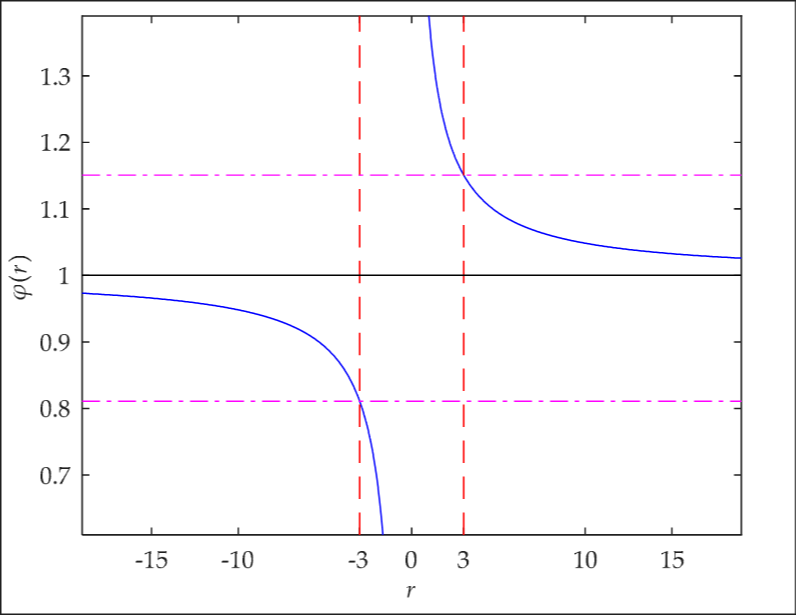
\includegraphics[width=\textwidth]{../img/phi_r.png}
    \end{columns}
\end{frame}

% ============================================
% SLIDE 9: Weighted FGF Proposed Solution
% ============================================
\begin{frame}{Proposed Improvement: Weighted FGF}
    \textbf{Idea:} Since $\varphi(r) \approx 1$ for pixels in the star spot (high SNR), we can reclaim robustness by adding a weight $I_i$ to the logarithmic residual.
    
    \vspace{0.2cm}
    \textbf{New Objective Function $H$:}
    \[
    H = \operatorname*{argmin}_{\mathbf{v}} \sum_{i \in U} \left[ I_i (\ln I_i - \ln S_i) \right]^2 
      = \operatorname*{argmin}_{\mathbf{v}} \sum_{i \in U} \left[ \varphi(r_i) N_i \right]^2
    \]
    
    \vspace{0.2cm}
    \textbf{Why this works:}
    \begin{itemize}
        \item $U$ is the set of pixels where $\varphi(r) \approx 1$ (the star spot).
        \item This effectively acts as a \textbf{Weighted GF} where the weight of each pixel is determined by $\varphi(r_i)$.
        \item Since $\varphi(r_i) \approx 1$ for the star, this equation approximates the standard GF, recovering optimal noise robustness while maintaining the speed of the logarithmic formulation.
    \end{itemize}
\end{frame}

% ============================================
% SLIDE 10: Linearizing the Weighted Model
% ============================================
\begin{frame}{Derivation: Linearizing the Weighted Model}
    Substituting the Gaussian model into the weighted objective function implies:
    \vspace{0.5cm}
    \begin{columns}[T]
        \column{0.55\textwidth}
        \textbf{Linearized Objective Function $H$:}
        \scriptsize
        \begin{align*}
            H &= \operatorname*{argmin}_{\mathbf{v}} \sum_{i \in U} \left( 
            m I_i x_i^2 + n I_i y_i^2 + \right. \\
            &\quad \left. p I_i x_i + q I_i y_i + k I_i + I_i \ln I_i 
            \right)^2 \\
            &= \operatorname*{argmin}_{\mathbf{m}} \sum_{i \in U} h_i^2
        \end{align*}
        
        \column{0.45\textwidth}
        \textbf{Parameter Substitution:}
        \scriptsize
        \begin{align*}
            m &= \frac{1}{2\sigma_x^2}, \quad n = \frac{1}{2\sigma_y^2} \\
            p &= -\frac{x_c}{\sigma_x^2}, \quad q = -\frac{y_c}{\sigma_y^2} \\
            k &= \frac{x_c^2}{2\sigma_x^2} + \frac{y_c^2}{2\sigma_y^2} - \ln A
        \end{align*}
    \end{columns}
    
    \vspace{0.3cm}
    \textbf{Result:} A standard \textbf{Linear Least Squares} problem for variables $m,n,p,q,k$.
\end{frame}

% ============================================
% SLIDE 11: Solution and Parameter Recovery
% ============================================
\begin{frame}{Solution and Parameter Recovery}
    \begin{columns}[T]
        \column{0.5\textwidth}
        \textbf{1. Solve Linear System $\nabla H = 0$:}
        \scriptsize
        \begin{align*}
            \frac{\partial H}{\partial m} &= \sum_{i \in U} 2 I_i x_i^2 h_i = 0 \\
            \frac{\partial H}{\partial n} &= \sum_{i \in U} 2 I_i y_i^2 h_i = 0 \\
            \frac{\partial H}{\partial p} &= \sum_{i \in U} 2 I_i x_i h_i = 0 \\
            \frac{\partial H}{\partial q} &= \sum_{i \in U} 2 I_i y_i h_i = 0 \\
            \frac{\partial H}{\partial k} &= \sum_{i \in U} 2 I_i h_i = 0
        \end{align*}
        
        \column{0.5\textwidth}
        \textbf{2. Recover Physical Parameters:}
        \scriptsize
        \begin{align*}
            x_c &= - \frac{p}{2m} \\[1em]
            y_c &= - \frac{q}{2n} \\[1em]
            \sigma_x &= \frac{1}{\sqrt{2m}}, \quad \sigma_y = \frac{1}{\sqrt{2n}} \\[1em]
            A &= \exp\left( \frac{p^2}{4|m|} + \frac{q^2}{4|n|} - k \right)
        \end{align*}
    \end{columns}
    
    \vspace{0.2cm}
    \begin{block}{Validity Condition}
        The approximation relies on $\varphi(r_i) \approx 1$. Thus, we must \textbf{threshold based on SNR} to define the set $U$.
    \end{block}
\end{frame}

% ============================================
% SLIDE 12: Two-Step Weighted FGF Algorithm
% ============================================
\begin{frame}{Algorithm: Two-Step Weighted FGF}
    \begin{algorithm}[H]
    \scriptsize
    \caption{Two-Step Weighted Fast Gaussian Fitting}
    \begin{algorithmic}[1]
        \REQUIRE Star Spot $\mathcal{S}$, Threshold $T_{\text{SNR}}$
        \ENSURE Centroid $(x_c, y_c)$
        \IF{$\text{PixelCount}(\mathcal{S}) < 5$ \OR $\text{HasSaturatedPixels}(\mathcal{S})$}
            \RETURN \textbf{null}
        \ENDIF
        \STATE $U_{\text{init}} \gets \text{SelectBrightestPixels}(\mathcal{S}, n=5)$ \quad \textit{// Assumes high SNR}
        \STATE $\mathbf{v}' \gets \text{SolveWeightedFGF}(U_{\text{init}})$ \quad \textit{// Rough params $(A', x_c', \dots)$}
        \FOR{\textbf{each} pixel $i \in \mathcal{S}$}
            \STATE $\hat{S}_i \gets \text{EvaluateGaussian}(i, \mathbf{v}')$; 
            \STATE $\hat{N}_i \gets I_i - \hat{S}_i$
            \STATE $r_i \gets |\hat{S}_i / \hat{N}_i|$
        \ENDFOR
        \STATE $U_{\text{final}} \gets \{ i \in \mathcal{S} \mid r_i > T_{\text{SNR}} \}$ \quad \textit{// Strictly satisfy $\varphi(r) \approx 1$, choice of $T_{\text{SNR}}$ is critical}
        \STATE $\mathbf{v}_{\text{final}} \gets \text{SolveWeightedFGF}(U_{\text{final}})$ \quad \textit{// Final Linear Least Squares}
        \RETURN $(x_c, y_c)$ \textbf{from} $\mathbf{v}_{\text{final}}$
    \end{algorithmic}
    \end{algorithm}
\end{frame}

% ============================================
% SLIDE 13: Experimental Setup
% ============================================
\begin{frame}{Experimental Setup}
    \textbf{Simulated Star Images:}
    \begin{itemize}
        \item Size: $31 \times 31$ pixels, single star spot.
        \item Model: Gaussian distribution + Gaussian noise ($\mu=0, \sigma_g$).
    \end{itemize}

    \vspace{0.3cm}
    \textbf{Algorithm Parameter Selection:}
    \begin{block}{Threshold Selection ($T$)}
        They selected \textbf{$T=3$} to balance two conflicting requirements:
        \begin{enumerate}
            \item \textbf{Sample Size:} Set $U$ must have $\ge 5$ pixels for fitting.
            \item \textbf{SNR Requirement:} $\varphi(r)$ must be close to 1 (high SNR) for selected pixels.
        \end{enumerate}
        \small $T=3$ ensures robust selection across diverse star conditions.
    \end{block}
\end{frame}

% ============================================
% SLIDE 14: Accuracy Results (Position & Radius)
% ============================================
\begin{frame}{Accuracy: Spot Position \& Radius}
    \begin{columns}
        \column{0.5\textwidth}
        \centering
        \textbf{1. Systematic Error (S-Curve)}
        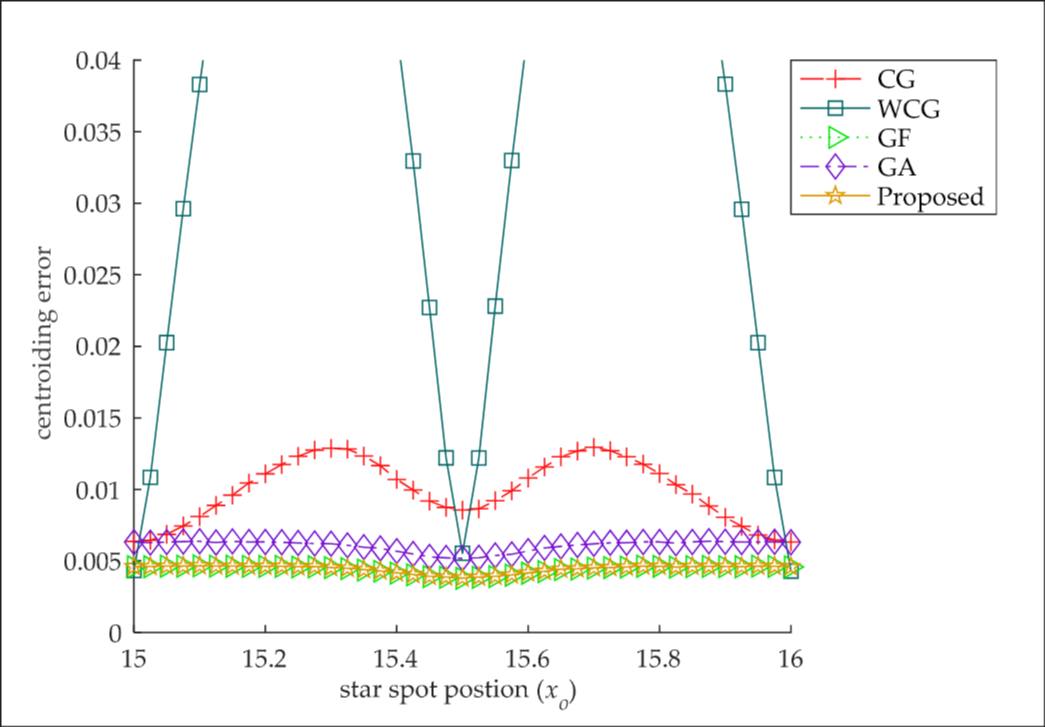
\includegraphics[width=0.9\textwidth]{../img/figure_4.png}
        \begin{itemize}
            \item \textbf{CG/WCG:} Significant S-curve error (pixel locking).
            \item \textbf{Fitting (GF/FGF):} \textbf{No systematic error}.
        \end{itemize}

        \column{0.5\textwidth}
        \centering
        \textbf{2. Impact of Spot Radius ($\sigma_r$)}
        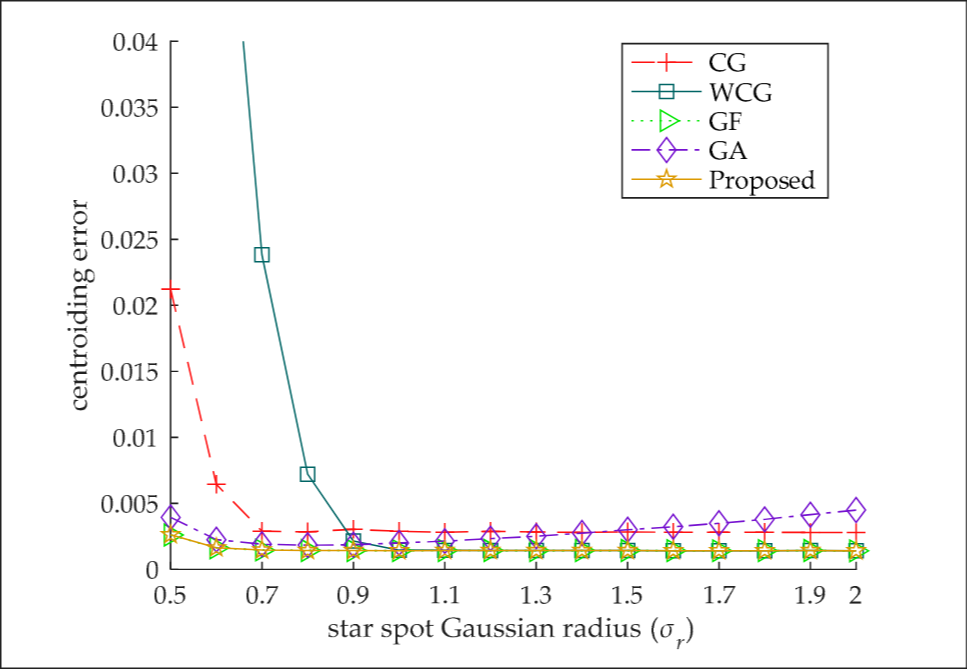
\includegraphics[width=0.9\textwidth]{../img/figure_5.png}
        \begin{itemize}
            \item \textbf{All Methods:} Error stable when $\sigma_r > 0.8$.
            \item \textbf{FGF (Proposed):} Matches \textbf{GF accuracy} perfectly, beating GA/CG.
        \end{itemize}
    \end{columns}
\end{frame}

% ============================================
% SLIDE 15: Accuracy Results (Noise & Brightness)
% ============================================
\begin{frame}{Accuracy: Noise \& Brightness}
    \begin{columns}
        \column{0.5\textwidth}
        \centering
        \textbf{3. Impact of Noise ($\sigma_g$)}
        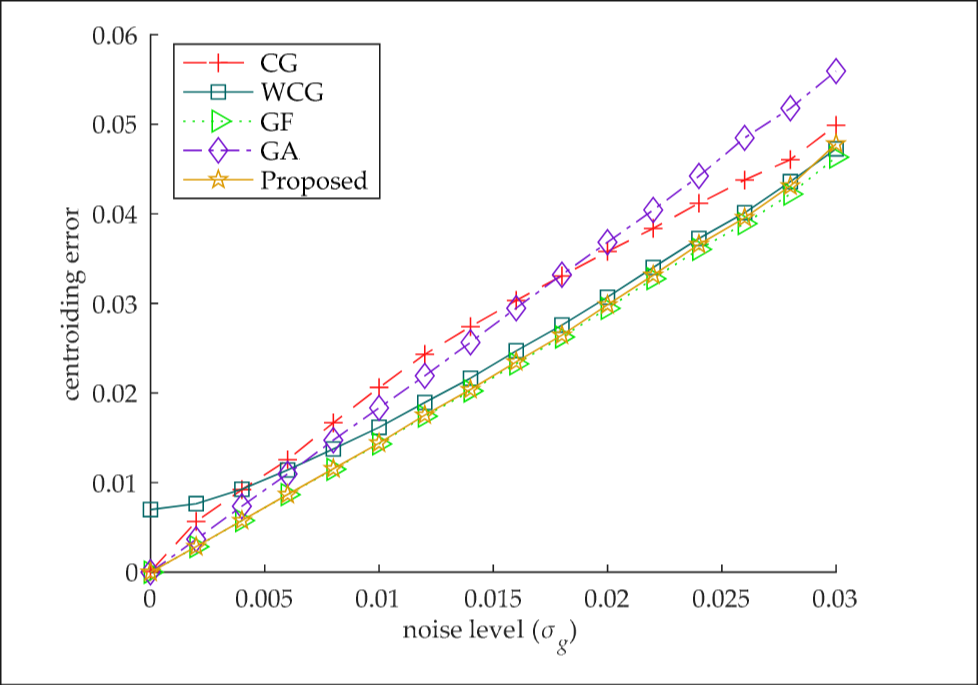
\includegraphics[width=0.9\textwidth]{../img/figure_6.png}
        \begin{itemize}
            \item \textbf{Trend:} Error increases linearly with noise.
            \item \textbf{Result:} FGF is \textbf{most robust}, overlapping with GF. Outperforms CG/GA significantly at high noise.
        \end{itemize}

        \column{0.5\textwidth}
        \centering
        \textbf{4. Impact of Brightness ($A$)}
        \includegraphics[width=0.9\textwidth]{../img/figure_7.png}
        \begin{itemize}
            \item \textbf{Saturation:} CG/WCG fail when pixels saturate ($A > 1$).
            \item \textbf{FGF/GF:} \textbf{Unaffected} by saturation (robust exclusion of saturated pixels).
        \end{itemize}
    \end{columns}
\end{frame}

% ============================================
% SLIDE 16: Efficiency Comparison
% ============================================
\begin{frame}{Efficiency Comparison}
    \textbf{Total Time Consumption (10,000 images):}
    
    \begin{table}
        \centering
        \begin{tabular}{lr}
            \toprule
            \textbf{Method} & \textbf{Time (s)} \\
            \midrule
            Center of Gravity (CG) & \textbf{1.35 s} \\
            Weighted CG (WCG) & 1.39 s \\
            Gaussian Analytical (GA) & 1.49 s \\
            \textbf{Proposed (FGF)} & \textbf{3.97 s} \\
            Gaussian Fitting (GF) & 58.99 s \\
            \bottomrule
        \end{tabular}
    \end{table}
    
    \vspace{0.3cm}
    \textbf{Analysis:}
    \begin{itemize}
        \item \textbf{FGF vs GF:} $\sim \mathbf{15\times}$ \textbf{faster} than standard iterative GF.
        \item \textbf{FGF vs CG:} Only $\sim 3\times$ slower than the simplest method.
        \item \textbf{Trade-off:} FGF provides \textbf{GF-level accuracy} at near-CG speed.
    \end{itemize}
\end{frame}

% ============================================
% SLIDE 17: Conclusion
% ============================================
\begin{frame}{Conclusion}
    \begin{block}{Summary}
        The proposed \textbf{Fast Gaussian Fitting (FGF)} algorithm solves the bias problem of standard linearization by introducing a \textbf{two-step SNR-weighted approach}.
    \end{block}
    
    \vspace{0.3cm}
    \textbf{Key Achievements:}
    \begin{enumerate}
        \item \textbf{Accuracy:} Matches the theoretical optimum (GF) and is robust to S-curve error, high noise, and saturation.
        \item \textbf{Speed:} Significantly faster than iterative methods, suitable for real-time applications (approx. 4ms per 10k images).
        \item \textbf{Robustness:} Analytic SNR-thresholding explicitly handles weight nonuniformity.
    \end{enumerate}
    
    \vspace{0.3cm}
    \centering
\end{frame}

% ============================================
% PART 2: Implementation
% ============================================
\section{Rust Autoguider Implementation}

% ============================================
% SLIDE 18a: Context - The Tracking Challenge
% ============================================
\begin{frame}{Context: The Tracking Challenge}
    \begin{columns}
        \column{0.55\textwidth}
        \textbf{Problem:}
        In long-exposure astrophotography, stars must remain fixed on the sensor for minutes to avoid "star trails".
        
        \vspace{0.2cm}
        \textbf{Sources of Tracking Error:}
        \begin{itemize}
            \item \textbf{Earth Rotation:} Compensated by Equatorial Mounts that rotate counter to Earth at sidereal rate.
            \item \textbf{Polar Alignment Error:} Even slight misalignment of the mount's axis induces drift in \textbf{both Declination and Right Ascension}.
            \item \textbf{Periodic Error (PE):} Imperfections in the gears cause oscillating tracking speed.
            \item \textbf{Flexure \& Atmosphere:} Differential bending of the telescope and atmospheric refraction.
        \end{itemize}
        
        \column{0.45\textwidth}
        \centering
        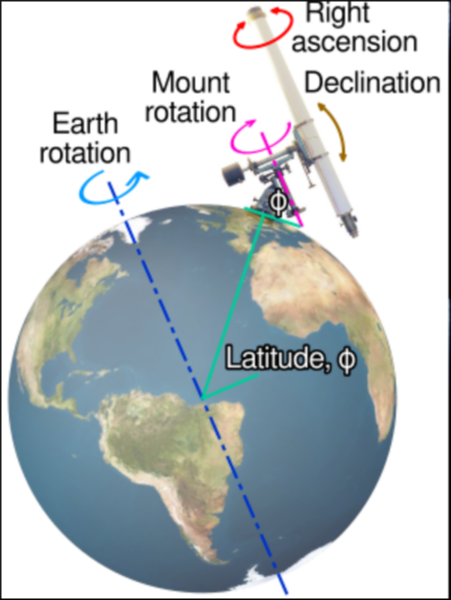
\includegraphics[width=0.75\textwidth]{../img/eq_mount.png}
    \end{columns}
\end{frame}

% ============================================
% SLIDE 18b: Context - The Autoguiding Solution
% ============================================
\begin{frame}{Context: The Autoguiding Solution}
    \begin{columns}
        \column{0.55\textwidth}
        \textbf{The Solution: Closed-Loop Control}
        Since open-loop tracking (blind correction) is insufficient for sub-arcsecond precision, we use an \textbf{Autoguider}.
        
        \vspace{0.3cm}
        \textbf{How it works:}
        \begin{enumerate}
            \item A secondary \textbf{Guide Scope} and camera are mounted in parallel to the main telescope.
            \item The camera tracks a "Guide Star" at high frequency (1-10Hz).
            \item The software measures the star's drift from its original lock position.
            \item Corrective pulses are sent to the mount motors to bring the star back to center.
        \end{enumerate}
        
        \column{0.45\textwidth}
        \centering
        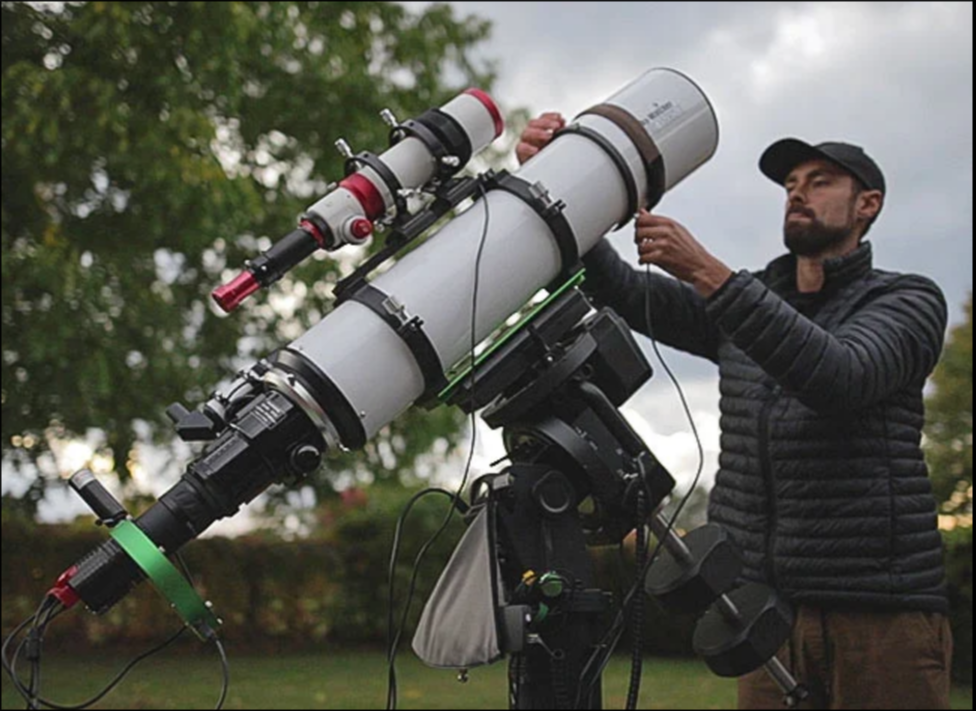
\includegraphics[width=0.9\textwidth]{../img/guide_scope.png}
        \vspace{0.1cm}
        \tiny \textit{Typical Setup: Main Imaging Scope (Large) + Guide Scope (Small, Top) with Camera }
    \end{columns}
\end{frame}

% ============================================
% SLIDE 19: System Architecture
% ============================================
\begin{frame}{System Architecture}
    \begin{columns}
        \column{0.6\textwidth}
        \textbf{Technology Stack:}
        \begin{itemize}
            \item \textbf{Language:} \textcolor{orange}{Rust} (Performance)
            \item \textbf{Runtime:} \texttt{Tokio} (Async event loop, 10Hz cycle)
            \item \textbf{Web Server:} \texttt{Axum} (Telemetry \& Control UI)
            \item \textbf{Math:} \texttt{Nalgebra} (Linear algebra for FGF)
        \end{itemize}
        
        \vspace{0.3cm}
        \textbf{Key Features:}
        \begin{itemize}
            \item \textbf{High Concurrency:} Image capturing, processing, and web serving run asynchronously.
            \item \textbf{Real-time Telemetry:} Full state (images + error graphs) pushed to frontend via \textbf{WebSockets}.
        \end{itemize}
        
        \column{0.4\textwidth}
        \centering
        \begin{tikzpicture}[node distance=1.2cm, scale=0.7, transform shape,
            block/.style={rectangle, draw, fill=blue!10, rounded corners, minimum width=2.5cm, minimum height=1cm, align=center},
            arrow/.style={thick, ->, >=stealth}
            ]
            \node[block, fill=stargold!20] (camera) {Simulated\\Camera};
            \node[block, below of=camera, yshift=-1.5cm] (backend) {\textbf{Rust Backend}\\(Guiding Loop)};
            \node[block, fill=green!10, below of=backend, yshift=-1.5cm] (web) {Web Frontend\\(HTML/JS)};
            
            \draw[arrow] (camera) -- node[right] {Raw Frames} (backend);
            \draw[arrow] (backend) -- node[right] {JSON/WS} (web);
            \draw[arrow] (web.west) -- ++(-0.5,0) |- node[midway, left] {Commands} (backend.west);
        \end{tikzpicture}
    \end{columns}
\end{frame}

% ============================================
% SLIDE 19a: Simulation Environment
% ============================================
\begin{frame}{Simulation Environment}
    To validate the autoguider without physical hardware, a **Virtual Camera** was implemented to simulate optics and atmosphere.

    \begin{columns}
        \column{0.6\textwidth}
        \textbf{1. Optic Rendering:}
        \begin{itemize}
            \item \textbf{Input:} High-resolution star field image.
            \item \textbf{Sub-pixel Drift:} Uses \textbf{Bilinear Interpolation} to render stars at non-integer coordinates $(x,y)$.
            \item \textbf{Sampling:} 4-neighborhood weighted average ($p_{00}, p_{10}, p_{01}, p_{11}$) ensuring smooth sub-pixel motion.
        \end{itemize}

        \vspace{0.3cm}
        \textbf{2. Atmospheric Simulation (Seeing):}
        \begin{itemize}
            \item \textbf{Scintillation:} Global brightness varies randomly by $\pm 10\%$ per frame ($I_{new} = I \cdot [0.9, 1.1]$).
            \item \textbf{Sensor Noise:} High-amplitude random noise is injected into every pixel ($\pm 20$ intensity units).
             \[ I_{\text{final}} = \operatorname{clamp}(I_{\text{interp}} \cdot \text{Flux}(t) + \text{Noise}) \]
        \end{itemize}

        \column{0.4\textwidth}
        \centering
        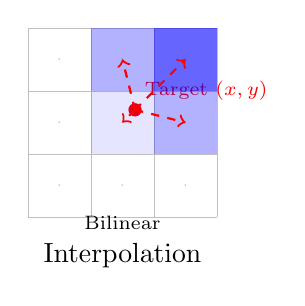
\begin{tikzpicture}[scale=0.8]
            % Pixel grid
            \draw[step=1cm,gray!50,very thin] (0,0) grid (3,3);
            % Pixels
            \foreach \x in {0.5, 1.5, 2.5}
                \foreach \y in {0.5, 1.5, 2.5}
                    \node[gray!50] at (\x,\y) {\tiny .};
            
            % Subpixel point
            \fill[red] (1.7, 1.7) circle (3pt) node[above right] {\scriptsize Target $(x,y)$};
            
            % Active pixels
            \fill[blue, opacity=0.1] (1,1) rectangle (2,2);
            \fill[blue, opacity=0.3] (2,1) rectangle (3,2);
            \fill[blue, opacity=0.3] (1,2) rectangle (2,3);
            \fill[blue, opacity=0.6] (2,2) rectangle (3,3);
            
            % Interpolation arrows
            \draw[->, red, dashed, thick] (1.7, 1.7) -- (1.5, 1.5);
            \draw[->, red, dashed, thick] (1.7, 1.7) -- (2.5, 1.5);
            \draw[->, red, dashed, thick] (1.7, 1.7) -- (1.5, 2.5);
            \draw[->, red, dashed, thick] (1.7, 1.7) -- (2.5, 2.5);
            
            \node[align=center] at (1.5, -0.4) {\scriptsize Bilinear\\Interpolation};
        \end{tikzpicture}
    \end{columns}
\end{frame}

% ============================================
% SLIDE 20: The Guiding Loop
% ============================================
\begin{frame}{The Guiding Loop (10Hz)}
    The system executes a classic closed-loop control cycle:
    
    \vspace{0.5cm}
    \centering
    \begin{tikzpicture}[auto, node distance=2cm, >=latex', scale=0.8, transform shape]
        % Styles
        \tikzstyle{block} = [draw, fill=blue!10, rectangle, minimum height=3em, minimum width=5em, rounded corners, align=center]
        \tikzstyle{sum} = [draw, fill=white, circle, node distance=1cm]
        \tikzstyle{input} = [coordinate]
        \tikzstyle{output} = [coordinate]

        % Nodes
        \node [input, name=input] {};
        \node [sum, right of=input, node distance=2.5cm] (sum) {$\Sigma$};
        \node [block, right of=sum, node distance=3.5cm, fill=green!10, text width=2.5cm] (controller) {\textbf{Controller}\\(Low Pass + PID)};
        \node [block, right of=controller, node distance=4.5cm, fill=red!10, text width=2.5cm] (plant) {\textbf{Mount}\\(Motors)};
        \node [output, right of=plant, node distance=3cm] (output) {};
        \node [block, below of=controller, node distance=2.5cm, fill=stargold!20, text width=3cm] (sensor) {\textbf{Sensor}\\(Camera + FGF)};
        
        % Disturbance
        \node [coordinate, above of=plant, node distance=1.5cm] (disturbance) {};

        % Connections
        \draw [thick, ->] (input) -- node[name=ref, above] {\small Setpoint ($0,0$)} (sum);
        \draw [thick, ->] (sum) -- node[above] {\small Error} (controller);
        \draw [thick, ->] (controller) -- node[above] {\small Pulse (ms)} (plant);
        \draw [thick, ->] (plant) -- node [name=y, near end, above] {\small Position} (output);
        \draw [thick, ->] (disturbance) -- node [right] {\small Drift/PE} (plant);
        
        % Feedback
        \draw [thick, ->] (y) |- (sensor);
        \draw [thick, ->] (sensor) -| node[pos=0.95, left] {\small $-$} (sum);
    \end{tikzpicture}
    
    \vspace{0.5cm}
    \begin{itemize}
        \item \textbf{Cycle Time:} 100ms (10Hz).
        \item \textbf{Input:} Desired centroid position (Locked).
        \item \textbf{Feedback:} Actual centroid position computed by \textbf{FGF}.
        \item \textbf{Disturbances:} Gear errors and atmospheric seeing are rejected by the loop.
    \end{itemize}
\end{frame}

% ============================================
% SLIDE 20: Star Selection & Robustness
% ============================================
\begin{frame}{Star Selection \& Robustness}
    Before guiding, the system must select reliable guide stars.
    
    \begin{columns}
        \column{0.5\textwidth}
        \textbf{Selection Criteria:}
        \begin{enumerate}
            \item \textbf{Brightness:} Must exceed noise floor.
            \item \textbf{Compactness:} Standard deviation of spatial variance $< 15.0$ (rejects galaxies/clouds).
            \item \textbf{Isolation:} Must be far from other bright sources.
        \end{enumerate}
        
        \vspace{0.3cm}
        \textbf{Outlier Rejection:}
        \begin{itemize}
            \item \textbf{Median Discrepancy Check:} If a star's movement deviates $>3$px from the group median, it is ignored (e.g., passing satellite).
        \end{itemize}
        
        \column{0.5\textwidth}
        \centering
        % Simple representation of selection
        \begin{tikzpicture}[scale=0.7]
            \fill[black] (0,0) rectangle (5,5);
            % Good stars
            \fill[stargold] (1,3) circle (0.15) node[above=2pt, white] {\tiny OK};
            \draw[green, thin] (1,3) circle (0.3);
            
            \fill[stargold] (3,4) circle (0.2) node[above=2pt, white] {\tiny OK};
            \draw[green, thin] (3,4) circle (0.35);
            
            % Bad star (Double/Galaxy)
            \fill[stargold!70] (2,1) ellipse (0.4 and 0.2);
            \node[red, below] at (2,0.7) {\tiny Reject (Not Compact)};
            \draw[red, thick] (1.5, 0.5) -- (2.5, 1.5);
            \draw[red, thick] (1.5, 1.5) -- (2.5, 0.5);
        \end{tikzpicture}
    \end{columns}
\end{frame}

% ============================================
% SLIDE 21: Control Logic (PID)
% ============================================
\begin{frame}{Control Logic: Filter \& PID}
    \textbf{1. Signal Filtering:}
    Raw centroid error is noisy. We apply a \textbf{First-order Low Pass Filter} (EMA) before the controller.
    \[
        E_{t} = \alpha \cdot E_{\text{raw}} + (1 - \alpha) \cdot E_{t-1}
    \]
    The smoothing factor $\alpha$ is derived dynamically from the cutoff frequency $f_c$:
    \[
        \alpha = \frac{\Delta t}{\Delta t + RC}, \quad \text{where } RC = \frac{1}{2\pi f_c}
    \]
    \small ($f_c \approx 0.05\text{Hz}$ for RA, $\Delta t = 0.1\text{s}$)
    \normalsize
    
    \vspace{0.2cm}
    \textbf{2. PID Controller:}
    Independent controllers for Right Ascension (RA) and Declination (DEC).
    \begin{itemize}
        \item \textbf{Proportional ($K_p$):} Immediate reaction to error.
        \item \textbf{Integral ($K_i$):} Corrects steady-state drift (e.g., polar misalignment) with \textbf{Anti-Windup} clamping.
        \item \textbf{Derivative ($K_d$):} Damping term to prevent oscillation.
    \end{itemize}
    
    \vspace{0.2cm}
    \textbf{Output:} Pulse duration (ms) sent to mount driver.
\end{frame}

% ============================================
% SLIDE 23: Algorithm Usage & Performance
% ============================================
\begin{frame}{Algorithm Usage \& Performance}
    \textbf{Real-Time Validation Strategy:}
    To rigorously evaluate the proposed FGF method, the autoguider software was designed to run \textbf{all three algorithms concurrently} on every frame:
    
    \begin{enumerate}
        \item \textbf{Control Path:} The \textbf{FGF} result drives the PID controller (ensuring low latency).
        \item \textbf{Validation Path:} \textbf{CoG} and \textbf{GF} run in parallel threads on the same data.
        \item \textbf{Telemetry:} Execution times and calculated centroids for all methods are logged to compare stability and speed under real sky conditions.
    \end{enumerate}

    \vspace{0.2cm}
    \textbf{Measured Execution Time (Rust Implementation):}
    \begin{table}
        \centering
        \begin{tabular}{l c c}
            \toprule
            \textbf{Algorithm} & \textbf{Implementation} & \textbf{Time per Star} \\
            \midrule
            \textbf{Center of Gravity} & Simple Iteration & $\sim 4 \mu s$ \\
            \textbf{FGF (Proposed)} & \texttt{nalgebra} Linear Solve & $\sim \mathbf{30 \mu s}$ \\
            \textbf{Gaussian Fit (NM)} & \texttt{argmin} Nelder-Mead & $\sim 2000 \text{--} 4000 \mu s$ \\
            \bottomrule
        \end{tabular}
    \end{table}
    
    \vspace{0.1cm}
    \small
    \textbf{Result:} FGF is \textbf{$\sim 100\times$ faster} than iterative GF, enabling high-frequency control (10Hz+) with moderate CPU usage.
\end{frame}

% ============================================
% SLIDE 24: Future Works
% ============================================
\begin{frame}{Future Works}
    While the current Rust autoguider validates the FGF algorithm in simulation, several steps remain for a full deployment:

    \begin{itemize}
        \item \textbf{Hardware Integration:}
        \begin{itemize}
            \item Connect to real mounts using the \textbf{INDI protocol} (Instrument Neutral Distributed Interface).
            \item The plate solver and camera control modules are already implemented and ready.
        \end{itemize}

        \item \textbf{Advanced Filtering:}
        \begin{itemize}
            \item Replace the simple controller with a \textbf{Kalman Filter}.
            \item Would allow predictive tracking of periodic errors (PE) rather than just reactive smoothing.
        \end{itemize}

        \item \textbf{Dithering Support:}
        \begin{itemize}
            \item Implement automatic dithering between exposures to reduce fixed-pattern noise in astrophotography.
            \item Requires coordination between the main imaging scope and the guide scope.
        \end{itemize}
        
    \end{itemize}
\end{frame}

% ============================================
% SLIDE 25: Final Conclusion
% ============================================
\begin{frame}{Final Presentation Conclusion}
    \begin{itemize}
        \item \textbf{Theory:} We demonstrated that Gaussian Fitting is optimal for accuracy, but slow.
        \item \textbf{Innovation:} \textbf{Weighted Fast Gaussian Fitting (FGF)} linearizes the problem while correcting for noise bias using SNR weights.
        \item \textbf{Implementation:} A complete \textbf{Rust-based Autoguider} was built.
        \item \textbf{Result:} The system achieves high-precision tracking ($< 0.3$ px RMS) with negligible computational load, validating FGF as a superior choice for embedded star trackers.
    \end{itemize}
\end{frame}

% ============================================
% SLIDE 26: Thank You
% ============================================
\begin{frame}{Thank You for your attention!}
    \centering
    \textbf{Some of my pictures}
    
    \begin{columns}[b]
        \column{0.65\textwidth}
        \centering
        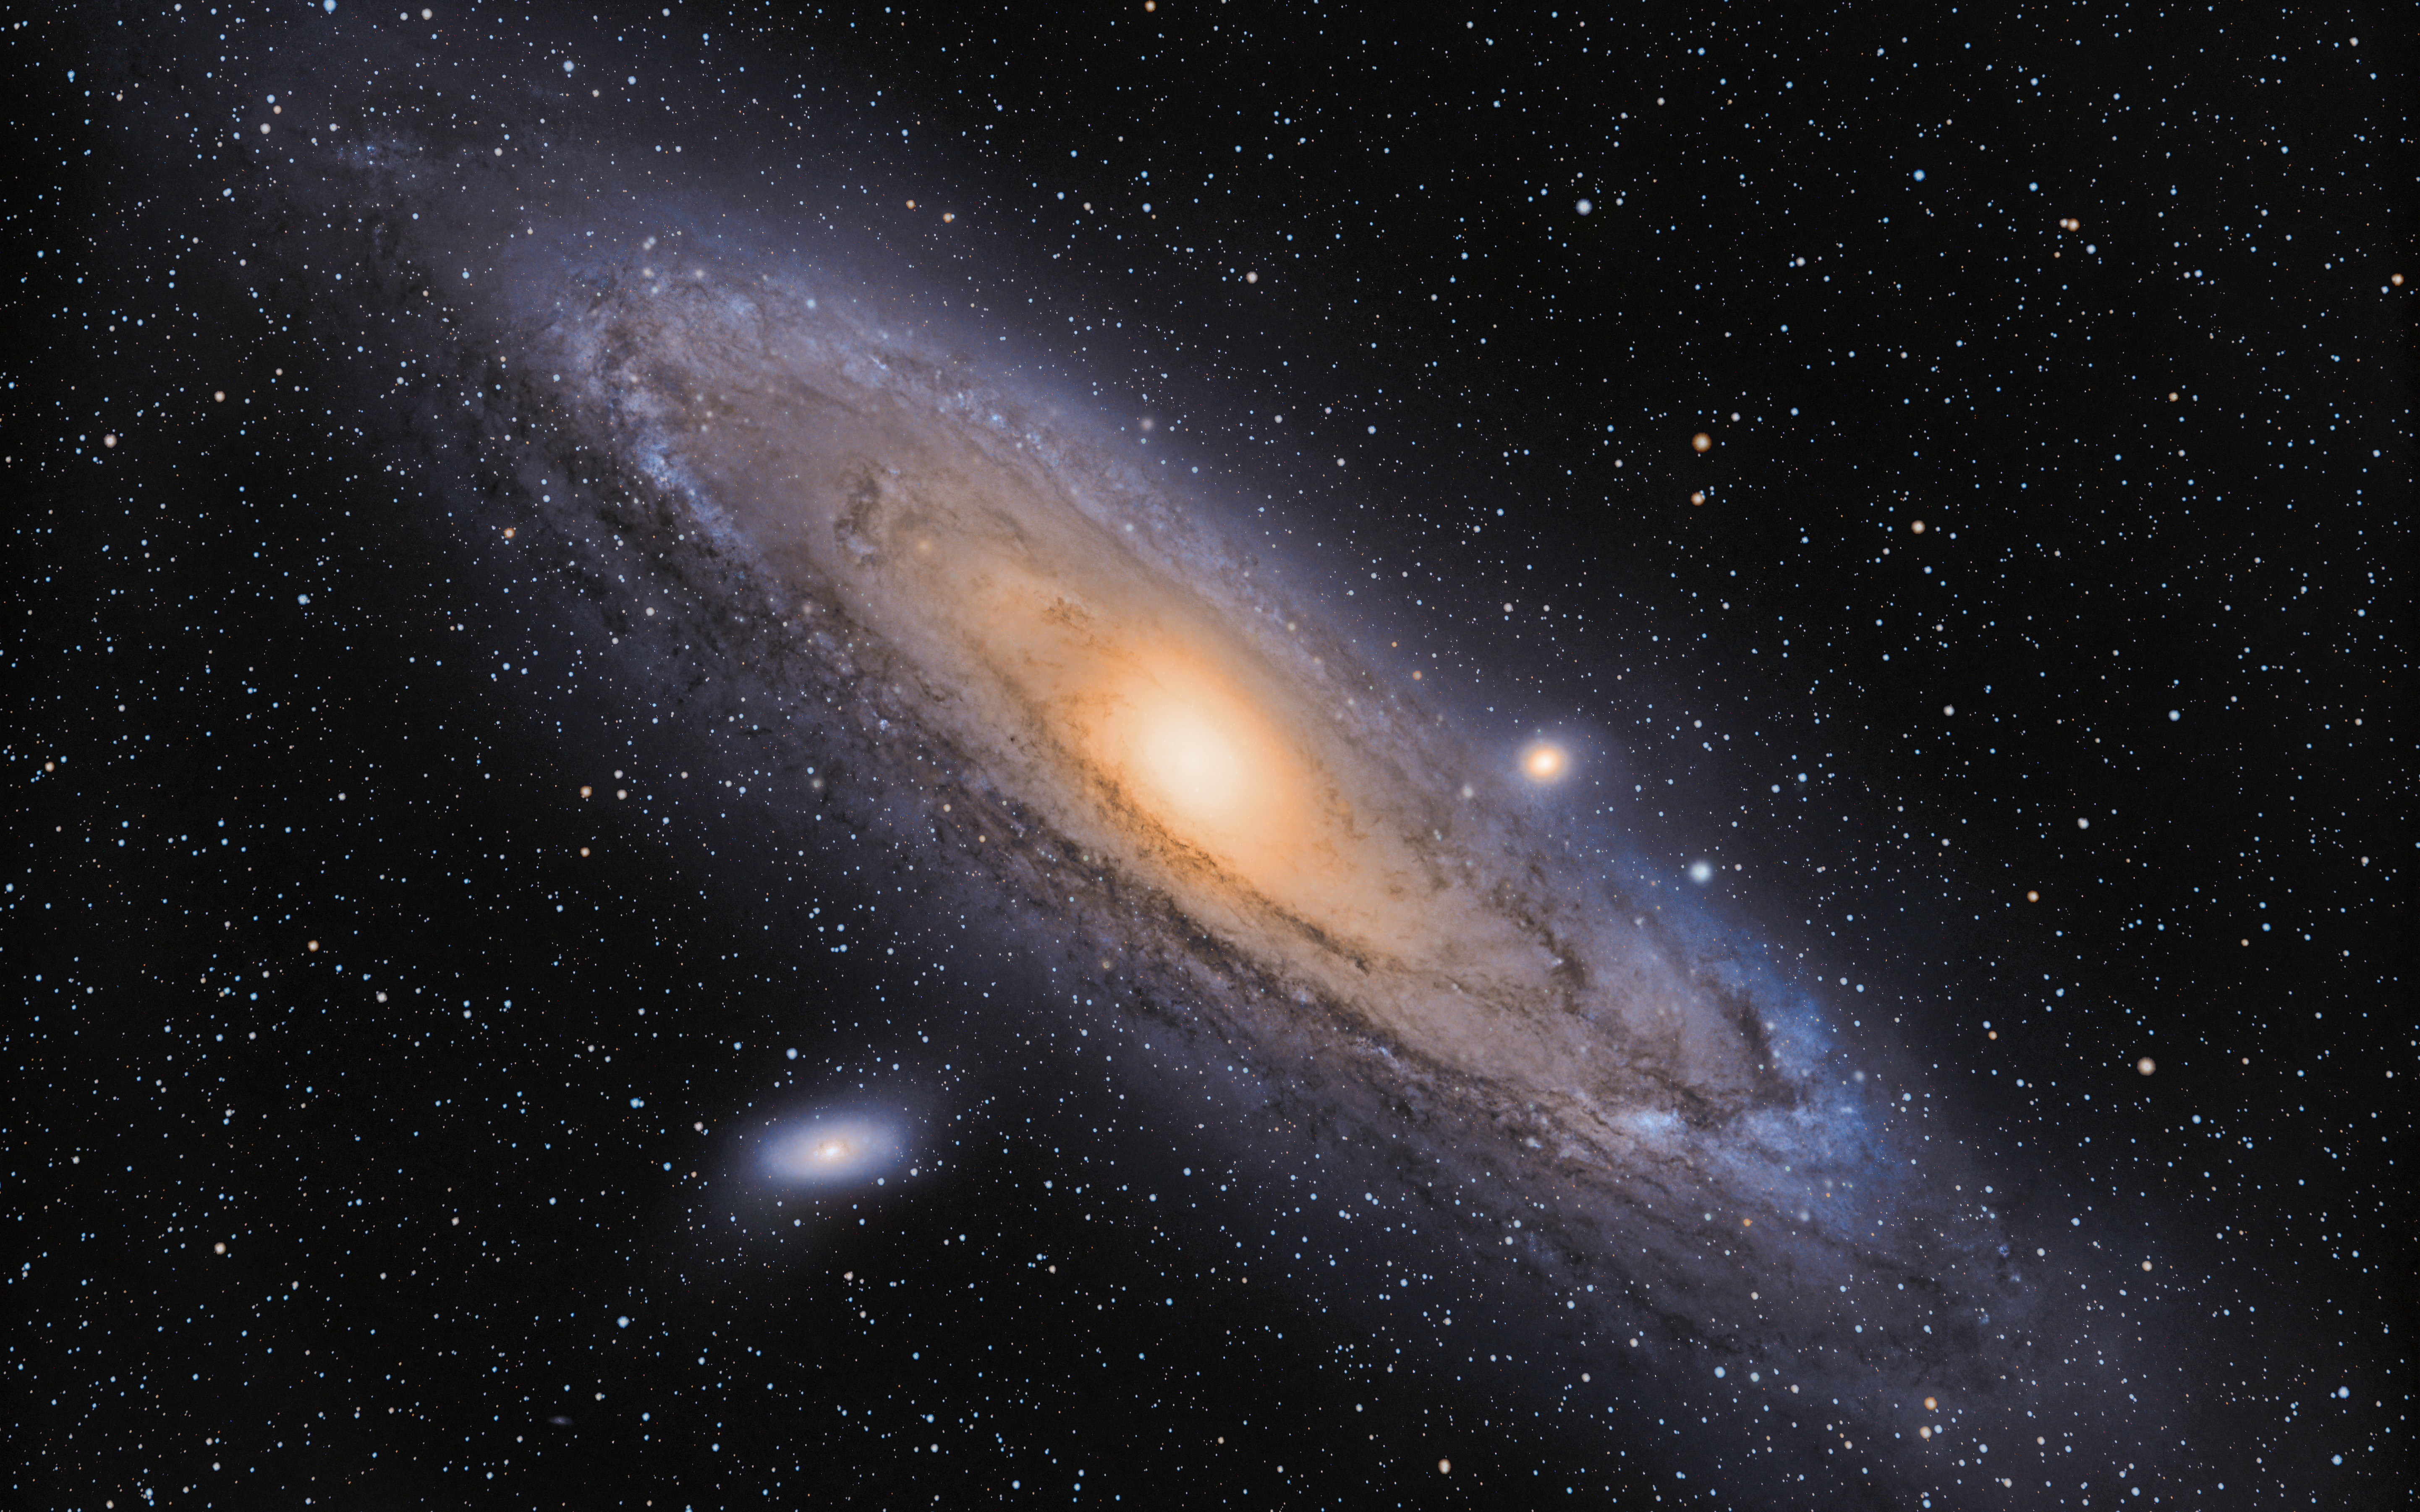
\includegraphics[width=1\textwidth]{../img/M31_Dimitry.D-1.jpg}
        \vspace{0.1cm}
        \tiny \textit{Andromeda Galaxy (M31)}
        
        \column{0.35\textwidth}
        \centering
        \includegraphics[width=1\textwidth]{../img/C33_C34_Dimitry.D-1.jpg}
        \vspace{0.1cm}
        \tiny \textit{The Veil Nebula (NGC 6960)}
    \end{columns}

\end{frame}


\appendix
\begin{frame}{Appendix: Matrix Formation}
    The minimization of $H$ leads to a system of 5 linear equations for the unknown vector $\mathbf{X} = [m, n, p, q, k]^T$. This can be written as $\mathbf{M}\mathbf{X} = \mathbf{Y}$.
    
    \vspace{0.2cm}
    \tiny
    \[
    \underbrace{
    \begin{bmatrix}
        \sum I_i^2 x_i^4 & \sum I_i^2 x_i^2 y_i^2 & \sum I_i^2 x_i^3 & \sum I_i^2 x_i^2 y_i & \sum I_i^2 x_i^2 \\
        \sum I_i^2 x_i^2 y_i^2 & \sum I_i^2 y_i^4 & \sum I_i^2 x_i y_i^2 & \sum I_i^2 y_i^3 & \sum I_i^2 y_i^2 \\
        \sum I_i^2 x_i^3 & \sum I_i^2 x_i y_i^2 & \sum I_i^2 x_i^2 & \sum I_i^2 x_i y_i & \sum I_i^2 x_i \\
        \sum I_i^2 x_i^2 y_i & \sum I_i^2 y_i^3 & \sum I_i^2 x_i y_i & \sum I_i^2 y_i^2 & \sum I_i^2 y_i \\
        \sum I_i^2 x_i^2 & \sum I_i^2 y_i^2 & \sum I_i^2 x_i & \sum I_i^2 y_i & \sum I_i^2
    \end{bmatrix}
    }_{\mathbf{M}}
    \underbrace{
    \begin{bmatrix}
        m \\ n \\ p \\ q \\ k
    \end{bmatrix}
    }_{\mathbf{X}}
    =
    \underbrace{
    \begin{bmatrix}
        -\sum I_i^2 x_i^2 \ln I_i \\ -\sum I_i^2 y_i^2 \ln I_i \\ -\sum I_i^2 x_i \ln I_i \\ -\sum I_i^2 y_i \ln I_i \\ -\sum I_i^2 \ln I_i
    \end{bmatrix}
    }_{\mathbf{Y}}
    \]
    \normalsize
    \vspace{0.2cm}
    The system is symmetric and can be solved efficiently (e.g., using LU decomposition).
\end{frame}

